\subsection{bpmrf/bpm\_\-rf.h File Reference}
\label{bpm__rf_8h}\index{bpmrf/bpm\_\-rf.h@{bpmrf/bpm\_\-rf.h}}


\subsubsection{Detailed Description}
libbpm rf simulation routines 

The header file for RF routines

Need to check in how far these routines are redundant, bpmdsp can replace most of the filtering routines here ! 

Definition in file {\bf bpm\_\-rf.h}.

{\tt \#include $<$math.h$>$}\par
{\tt \#include $<$bpm/bpm\_\-defs.h$>$}\par
{\tt \#include $<$bpm/bpm\_\-interface.h$>$}\par
{\tt \#include $<$bpm/bpm\_\-wf.h$>$}\par


Include dependency graph for bpm\_\-rf.h:\nopagebreak
\begin{figure}[H]
\begin{center}
\leavevmode
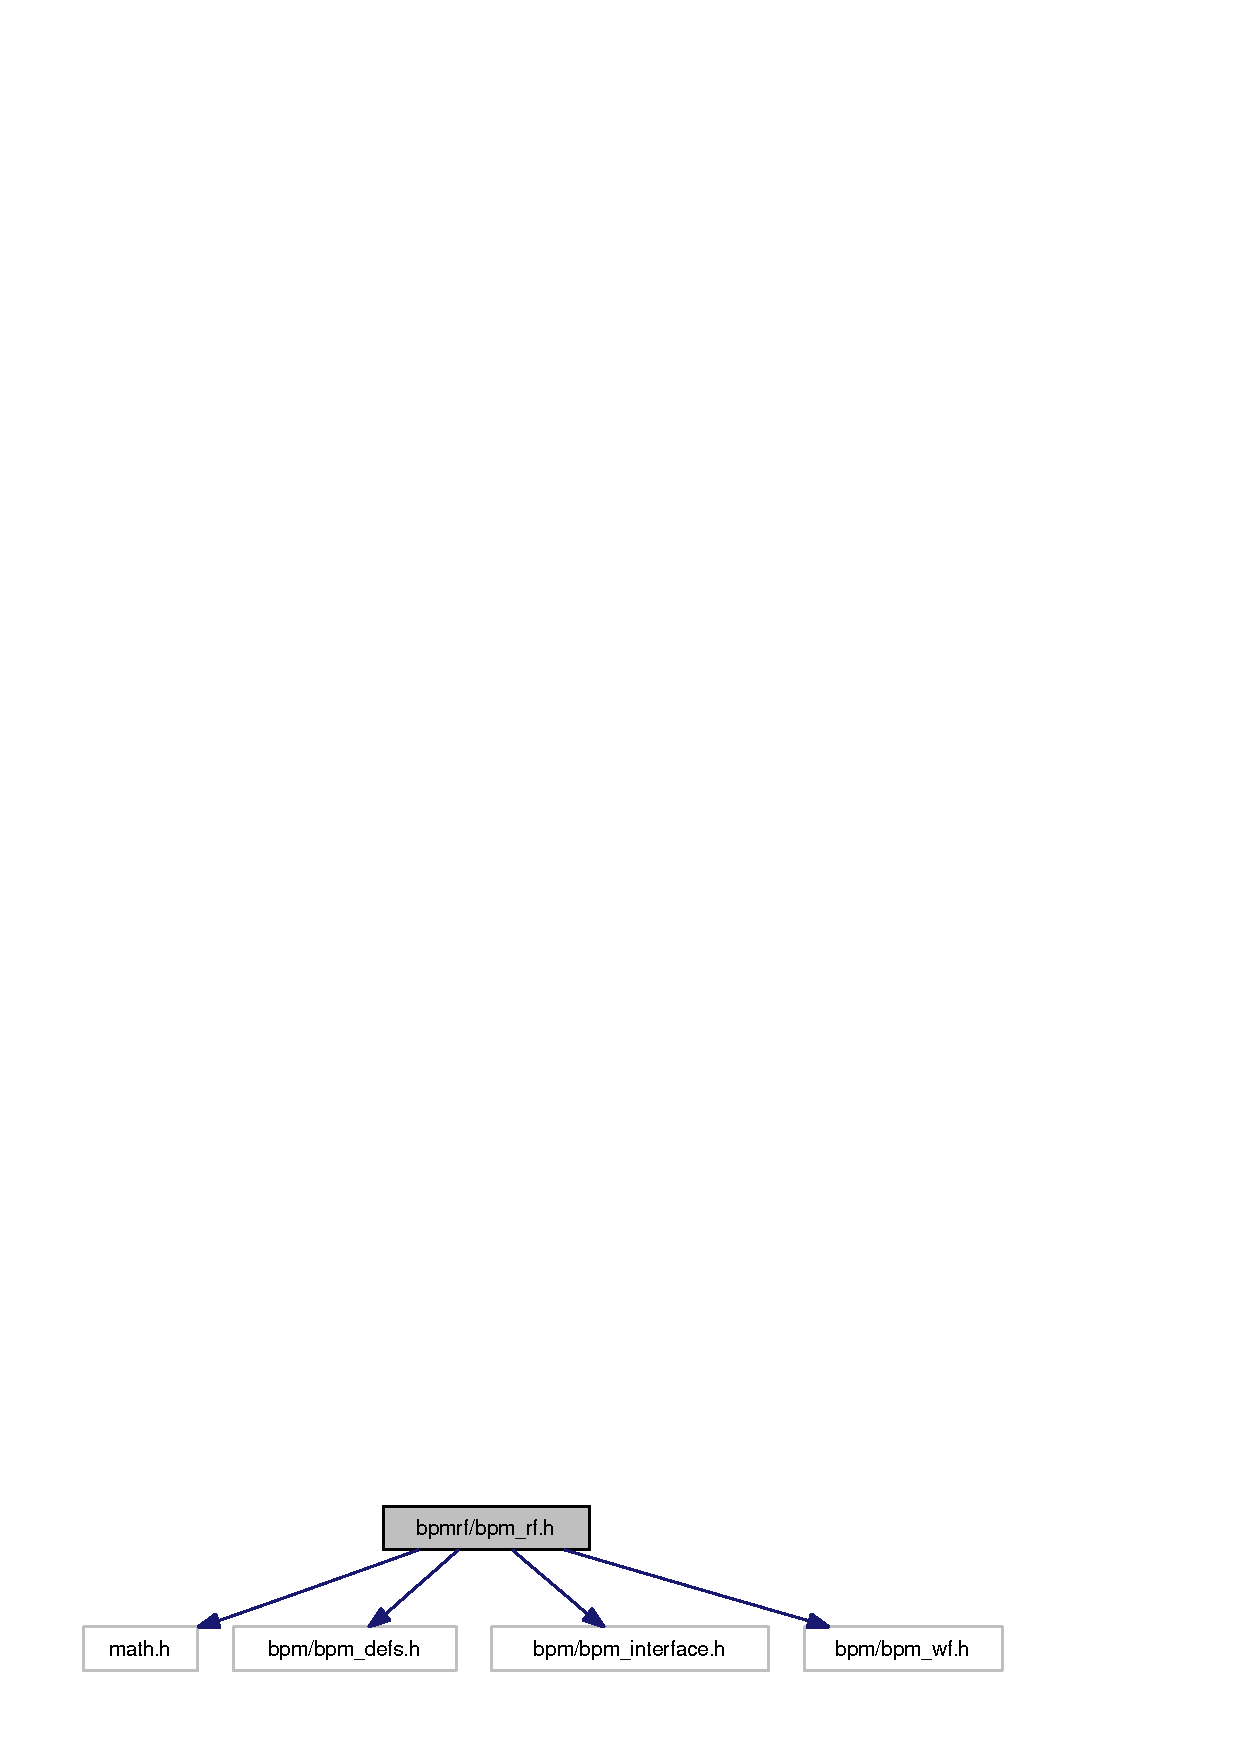
\includegraphics[width=242pt]{bpm__rf_8h__incl}
\end{center}
\end{figure}
\subsubsection*{Functions}
\begin{CompactItemize}
\item 
EXTERN int {\bf rf\_\-setup} (int nsamples, double sfreq)
\item 
EXTERN int {\bf rf\_\-rectify} ({\bf doublewf\_\-t} $\ast$D, {\bf complexwf\_\-t} $\ast$RF)
\item 
EXTERN int {\bf rf\_\-addLO} (double amp, double lofreq, enum {\bf bpmphase\_\-t} type, double phase, double phasenoise, {\bf doublewf\_\-t} $\ast$LO)
\item 
EXTERN int {\bf rf\_\-mixer} ({\bf doublewf\_\-t} $\ast$RF\_\-Re, {\bf doublewf\_\-t} $\ast$LO, {\bf doublewf\_\-t} $\ast$IF)
\item 
EXTERN int {\bf rf\_\-amplify} ({\bf doublewf\_\-t} $\ast$RF, double dB)
\item 
EXTERN int {\bf rf\_\-amplify\_\-complex} ({\bf complexwf\_\-t} $\ast$RF, double dB)
\item 
EXTERN int {\bf rf\_\-phase\_\-shifter} ({\bf complexwf\_\-t} $\ast$RF, double rotation)
\end{CompactItemize}
\subsubsection*{Variables}
\begin{CompactItemize}
\item 
EXTERN int {\bf rf\_\-nsamples}
\item 
EXTERN double {\bf rf\_\-samplefreq}
\end{CompactItemize}
